%% josis.tex 1.4   2016-09-15    JoSIS latex template
%------------------------------------------------------------------
% Filename: josis_template.tex
%
% This file is intended as a template for typesetting articles for the
%
%                        Journal of Spatial Information Science.
%
% Please edit this template to generate your own formatted manuscripts
% for submission to JOSIS. See http://josis.org for further details.
%


%%% JOSIS checks in typesetting
%%% * All titles and sections lower case *EXCEPT short title  [ ]
%%% * Remove author postal addresses, only have geographic places and institutions [ ] 
%%% * Consistent use of Section, Figure, Table (capitalized and in full) [ ]
%%% * 10 keywords (and all lower case) [ ]
%%% * Remove all avoidable footnotes [ ]
%%% * Use double quotation marks (``'' not "" or `') [ ]
%%% * Punctuation inside quotations [ ]
%%% * E.g. and i.e. followed by comma [ ]
%%% * cf. followed by tilde [ ]
%%% * Itemize and enumerate correctly punctuated [e.g., "1. x, 2. y, and 3. x." ]
%%% * And/or lists using American English punctuation (e.g., "x, y, and z") [ ] 
%%% * Bibliography (e.g., en-dashes for number ranges, consistent "Proc.~" for Proceedings of..., etc.) []
%%% * Acknowledgment style use section* [ ] 
%%% * et al. no italics, but with dot  [ ] 
%%% * All captions end with full stop  [ ] 
%%% * Table captions under, not over table  [ ]
%%% * Adjust urls with burlalt [ ] 
%%% * Check correct use of hyphens, emdashes, endashes  [ ]
%%% * Perform spell check  [ ] 

%%% JOSIS checks directly before publication 
%%% Check DOI, page numbers on article and web site. [ ]
%%% Update web site with final title, abstract, keywords. [ ] 
%%% Build with distiller for DOI links. [ ]


% Required documentclass definition for JOSIS
\documentclass{josis}
\usepackage{hyperref}
\usepackage{float}
\usepackage[hyphenbreaks]{breakurl}
\usepackage{booktabs}
\usepackage{stmaryrd}
\usepackage[T1]{fontenc}
\usepackage{cite}
\usepackage{subcaption}

% Suggested packages for algorithm formatting
\usepackage{algorithm}
%\usepackage{algorithmic}
\usepackage{algpseudocode}
\usepackage{pythonhighlight}

\usepackage{amssymb,amsmath}
%\usepackage[table]{xcolor}
\usepackage{lastpage}
\renewcommand{\topfraction}{0.9} 
\renewcommand{\textfraction}{0.1}
% Page setup and overhangs
\sloppy
\widowpenalty=10000
\clubpenalty=10000
\hyphenpenalty=75

% Article details for accepted manuscripts will be added by editorial staff
% Omit year if article in press
% Omit number if article under review
\josisdetails{%
   number=2, year=2024, firstpage=1, lastpage=\pageref{LastPage}, 
   doi={Technix}
  % received={December 24, 2015}, 
   %returned={February 25, 2016},
   %revised={July 13, 2016},
   %accepted={September 5, 2016},
   }

%\newcommand{\mydoi}[1]{\href{http://dx.doi.org/#1}{doi:\protect\detokenize{#1}}}

%\renewcommand{\UrlLeft}{http:\sslash}
%\DeclareUrlCommand\myurl{\def\UrlLeft{}\def\UrlRight{}%
%\urlstyle{tt}}

\urlstyle{rm}
\makeatletter
% Inspired by http://anti.teamidiot.de/nei/2009/09/latex_url_slash_spacingkerning/
% but slightly less kern and shorter underscore
\let\UrlSpecialsOld\UrlSpecials
\def\UrlSpecials{\UrlSpecialsOld\do\/{\Url@slash}\do\_{\Url@underscore}}%
\def\Url@slash{\@ifnextchar/{\kern-.11em\mathchar47\kern-.2em}%
    {\kern-.0em\mathchar47\kern-.08em\penalty\UrlBigBreakPenalty}}
\def\Url@underscore{\nfss@text{\leavevmode \kern.06em\vbox{\hrule\@width.3em}}}
\makeatother

\hypersetup{
colorlinks=true,
linkcolor=black,
citecolor=black,
urlcolor=black
} 

% Add the running author and running title information
\runningauthor{\begin{minipage}{.9\textwidth}\centering Rahul Biju,Nandakrishnan A,Nandana S Nair,Rahul Zachariah,Krishna Sagar P\end{minipage}}
\runningtitle{Running GenAI on Intel AI Laptops \& Simple LLM Inference on CPU \& fine-tuning of LLM Models using Intel\textsuperscript{\textregistered} OpenVINO\texttrademark}

% Document begins
\begin{document}
%\setcounter{page}{33}


% Insert your own title
\title{Running GenAI on Intel AI Laptops and Simple LLM Inference on CPU and fine-tuning of LLM Models using Intel\textsuperscript{\textregistered} OpenVINO\texttrademark}

% Insert your manuscipts authors, affiliations, and addresses
\author{Rahul Biju}
\author{Nandakrishnan A }
\author{Nandana S Nair}
\author{Rahul Zachariah}
\author{Krishna Sagar P}\affil{Saintgits Group of Institutions, Kottayam, Kerala}
\date{July 2024}
\maketitle
% Add 5-10 keywords for every submission
\keywords{TinyLlama, NNCF, LLM, CPU-based inference, Optimization, Intel\textregistered{} OpenVINO\texttrademark{} toolkit, Fine-tuning, Intel AI laptops, GenAI
}
% Add a short abstract of 150-250 words 
\begin{abstract}
This project optimizes large language models (LLMs) for efficient deployment on Intel AI laptops, focusing on CPU-based inference. It develops an advanced chatbot using the TinyLlama model, enhanced through Intel\textregistered{} OpenVINO\texttrademark{} toolkit and Neural Network Compression Framework (NNCF). The methodology demonstrates significant improvements in model size reduction and inference speed while maintaining performance. By quantizing and optimizing TinyLlama, the project showcases running sophisticated Gen AI models on consumer-grade hardware. This research contributes to democratizing Gen AI by making advanced language models accessible on widely available Intel platforms, highlighting the potential of running LLMs effectively on Intel CPUs.
\end{abstract}
% Your main text begins here. 
\section{Introduction}
The proliferation of large language models (LLMs) in AI has been constrained by their substantial computational demands. This project tackles the challenge of efficiently running sophisticated language models on consumer-grade Intel AI laptops, with a focus on CPU optimization. Utilizing the TinyLlama model and integrating Intel\textregistered{} OpenVINO\texttrademark{} technology with the Neural Network Compression Framework (NNCF), the project demonstrates a comprehensive optimization process for creating a text generation chatbot. The model undergoes conversion from PyTorch to ONNX format, transformation into OpenVINO Intermediate Representation (IR), and quantization for optimal performance. These steps significantly enhance the model's efficiency, reducing latency and improving inference speed while maintaining performance. Quantitative benchmarking using OpenVINO for CPU inference reveals notable improvements in model size and inference times. The optimized model is deployed in a Gradio interface, creating an interactive chatbot that showcases its enhanced capabilities. This research highlights the feasibility of running advanced AI models on widely accessible hardware, contributing to the democratization of AI technology.
\section{Literature Review}
Cazzaniga et al. [1] explore the impact of AI on the future of work, discussing economic, social, and ethical implications. They highlight AI's potential to enhance productivity while posing challenges for employment and income distribution, and emphasize the need for policies supporting workforce adaptation. Zhang et al. [2] introduce LLaMA-Adapter, a method for efficient fine-tuning of large language models using zero-initialized attention, achieving superior performance with reduced computational resources. This approach is especially relevant for scalable and cost-effective model adaptation. Lin et al. [3] propose a data-efficient fine-tuning framework for LLM-based recommendation systems, leveraging minimal data to improve recommendation accuracy. This method reduces computational burden, making fine-tuning accessible for applications with limited data. Church et al. [4] provide an overview of emerging trends in fine-tuning techniques, covering transfer learning and domain adaptation. They offer practical insights into implementing these methodologies, valuable for practitioners and researchers. Kustikova et al. [5] present a case study on using Intel\textregistered{} OpenVINO\texttrademark{} toolkit for semantic segmentation, highlighting its optimization capabilities for real-time AI applications. The study demonstrates the practical advantages of hardware-accelerated tools for improving inference efficiency and performance.


\section{Methodology}
In this work, a comprehensive methodology is followed for setting up and implementing an LLM chatbot using OpenVINO and other tools. The key stages in the implementation process are outlined below:
\subsection{Model selection and Model Preparation }
\begin{enumerate}
Model selection involves choosing the appropriate pre-trained model for a specific task. The TinyLlama/TinyLlama-1.1B-Chat-v1.0 model is chosen because it offers capabilities similar to larger models while requiring fewer computational resources. The preparation phase includes setting up the model and tokenizer, ensuring the model is ready for export, conversion, and optimization.
\end{enumerate}
\subsection{Model Conversion}
\begin{enumerate}
Converting a PyTorch model to OpenVINO involves first exporting the model to the ONNX format. The ONNX format serves as an intermediate representation that can be easily converted to the OpenVINO IR (Intermediate Representation) format. This conversion is crucial for optimizing the model to run efficiently on Intel hardware.
\end{enumerate}
\subsection{Model Optimisation}
\begin{enumerate}
The Neural Network Compression Framework (NNCF) in OpenVINO provides tools for optimizing models through techniques like quantization. Quantization reduces the precision of the model weights, leading to significant improvements in inference speed and reductions in model size without substantial loss in accuracy. The model is quantized using a performance preset, which balances speed and accuracy. The quantized model is then saved for later use.
\end{enumerate}
\subsection{CPU optimisation }
\begin{enumerate}
CPU optimization focuses on ensuring that the model runs efficiently on CPU hardware. This involves using optimized libraries and frameworks like OpenVINO, which are designed to fully leverage CPU capabilities. By converting and quantizing the model with OpenVINO, it utilizes Intel\textsuperscript{\textregistered}'s optimized inference engine, leading to better performance on CPUs compared to the original PyTorch model.
\end{enumerate}
\subsection{Inference and Benchmarking}
\begin{enumerate}
Inference and benchmarking involve running the model on sample inputs and measuring its performance. This includes calculating the average inference time and memory usage for both the original and quantized models. By comparing these metrics, the effectiveness of the optimizations can be determined. The quantized model is expected to show reduced inference time and memory size, indicating successful optimization.
\end{enumerate}

\subsection{User Interface}
\begin{enumerate}
The project utilizes Gradio to create a web-based interface, featuring a text input box, response display area, title, description, and sample prompts. This user-friendly design enables easy interaction with the TinyLlama model, allowing users to input text and receive generated responses without technical expertise.
\end{enumerate}


\section{Implementation}
Initially, the environment is set up with the necessary dependencies, including libraries such as "torch", "transformers", "openvino" and "nncf", alongside some standard Python libraries. The model chosen for this project is the TinyLlama/TinyLlama-1.1B-Chat-v1.0, a compact and efficient model suitable for conversational tasks.

The model and tokenizer are first initialized from Hugging Face's pre-trained weights, specifically using the Llama tokenizer for tokenization. After tokenization, "LlamaForCausalLM" from "transformers" is used to convert the tokenized model into a format that can be manipulated and used within the PyTorch framework. The model is then exported to ONNX format, which is a standard format for deep learning models that allows interoperability between different frameworks

Subsequently, the model has been exported to the OpenVINO Intermediate Representation (IR) format using the OpenVINO Core, consisting of an XML file describing the model architecture and a BIN file containing the model weights. These files are optimized for deployment on Intel hardware. A simple dataset class is defined to provide calibration data for quantization. This dataset class simulates a small set of input data to be used for calibrating the model's parameters during quantization. A hundred instances of the dummy input are used to create the calibration dataset.

The configuration defines a quantization process using NNCF (Neural Network Compression Framework) aimed at enhancing performance. The compression algorithm is set to quantization with a performance preset, aiming to balance speed and accuracy. The quantizer settings specify 8-bit precision for both weights and activations, utilizing an asymmetric quantization mode. This aggressive quantization approach aims to optimize the model's performance without significantly compromising its accuracy. The quantized model is serialized and saved in the output directory as an OpenVINO IR file. 


The preprocessing function "preprocess\_text" transforms the input text into a format suitable for the model by performing several steps. It first converts all characters to lowercase to ensure uniformity. Next, it removes all punctuation using the translate method and a translation table, effectively cleaning the text. Finally, it consolidates multiple spaces into a single space by splitting the text into words and rejoining them with a single space. This results in a cleaned and normalized text ready for the model to process.

The postprocessing function "postprocess\_response" refines the model's output to ensure it is well-formed and readable. It starts by trimming any leading or trailing whitespace from the response. Then, it splits the response into sentences using a regular expression that identifies sentence boundaries, ensuring that abbreviations and initials are not incorrectly split. Each sentence is then capitalized to maintain proper grammatical structure. Finally, the sentences are rejoined into a single string, resulting in a polished and coherent response suitable for presentation to the user.

The setup creates a Gradio interface for the TinyLlama Chatbot, designed to process user inputs and generate responses. The interface is configured to take text input from users through a textbox and display the chatbot's responses in another textbox.A pipeline has been used with task text generation for generating responses from the optimised TinyLlama model. This pipeline integrates seamlessly with the Gradio interface, handling the text generation process efficiently within the user interaction flow. When launched, the interface becomes publicly accessible and shareable, enabling users to interact with the TinyLlama Chatbot easily. Figure 1. shows the Gradio Interface of the TinyLlama Chatbot.

\begin{figure}[H]
\centering
\begin{subfigure}[b]{0.45\textwidth}
    \centering
    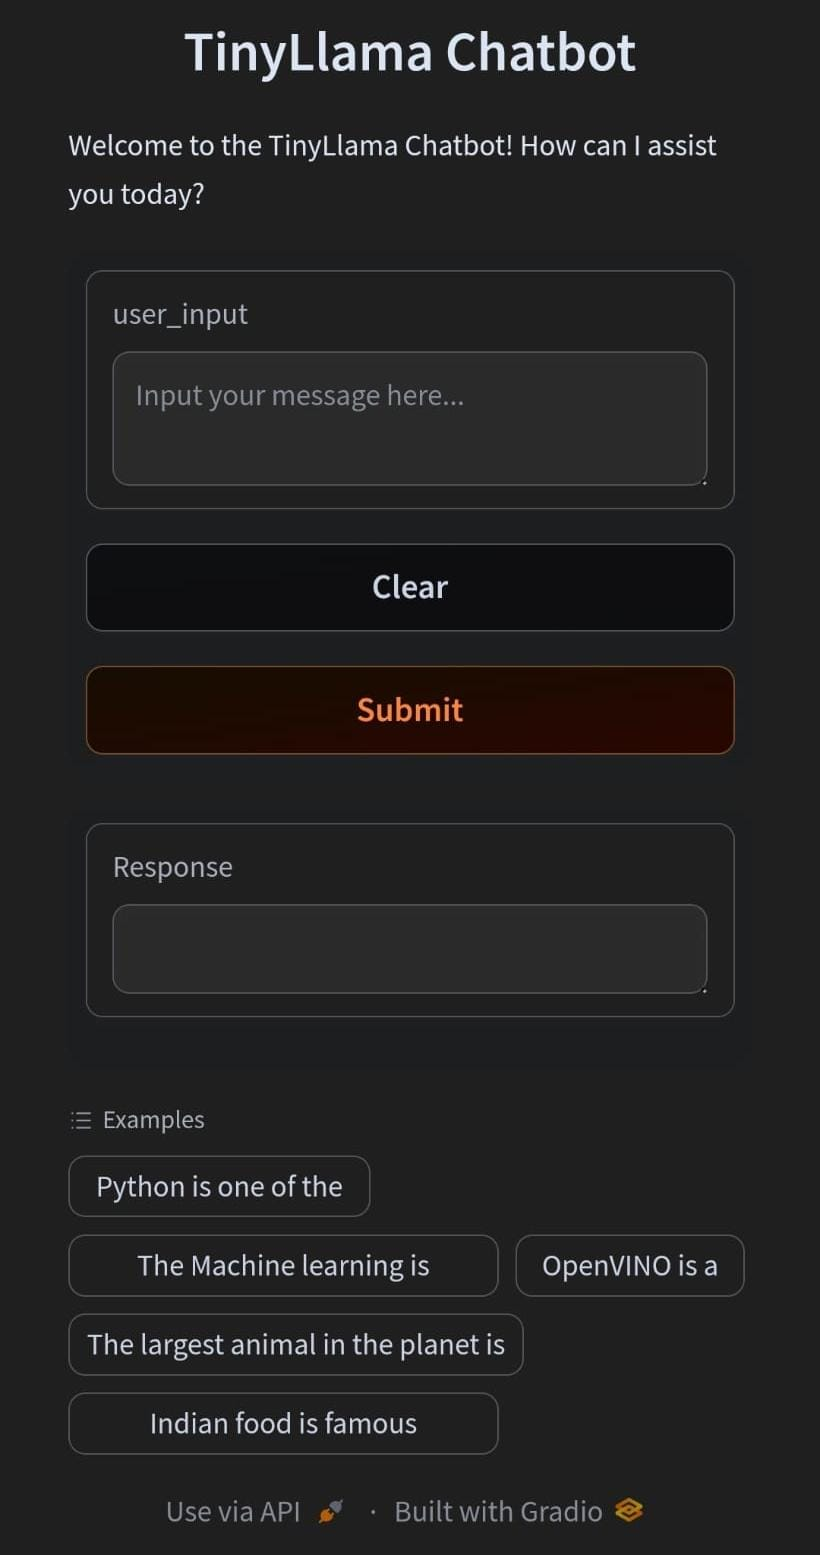
\includegraphics[width=\textwidth]{cove.jpg}
    \caption{Chatbot Interface}
    \label{fig:inference}
\end{subfigure}
% Add your second subfigure here if needed
\begin{subfigure}[b]{0.45\textwidth}
    \centering
    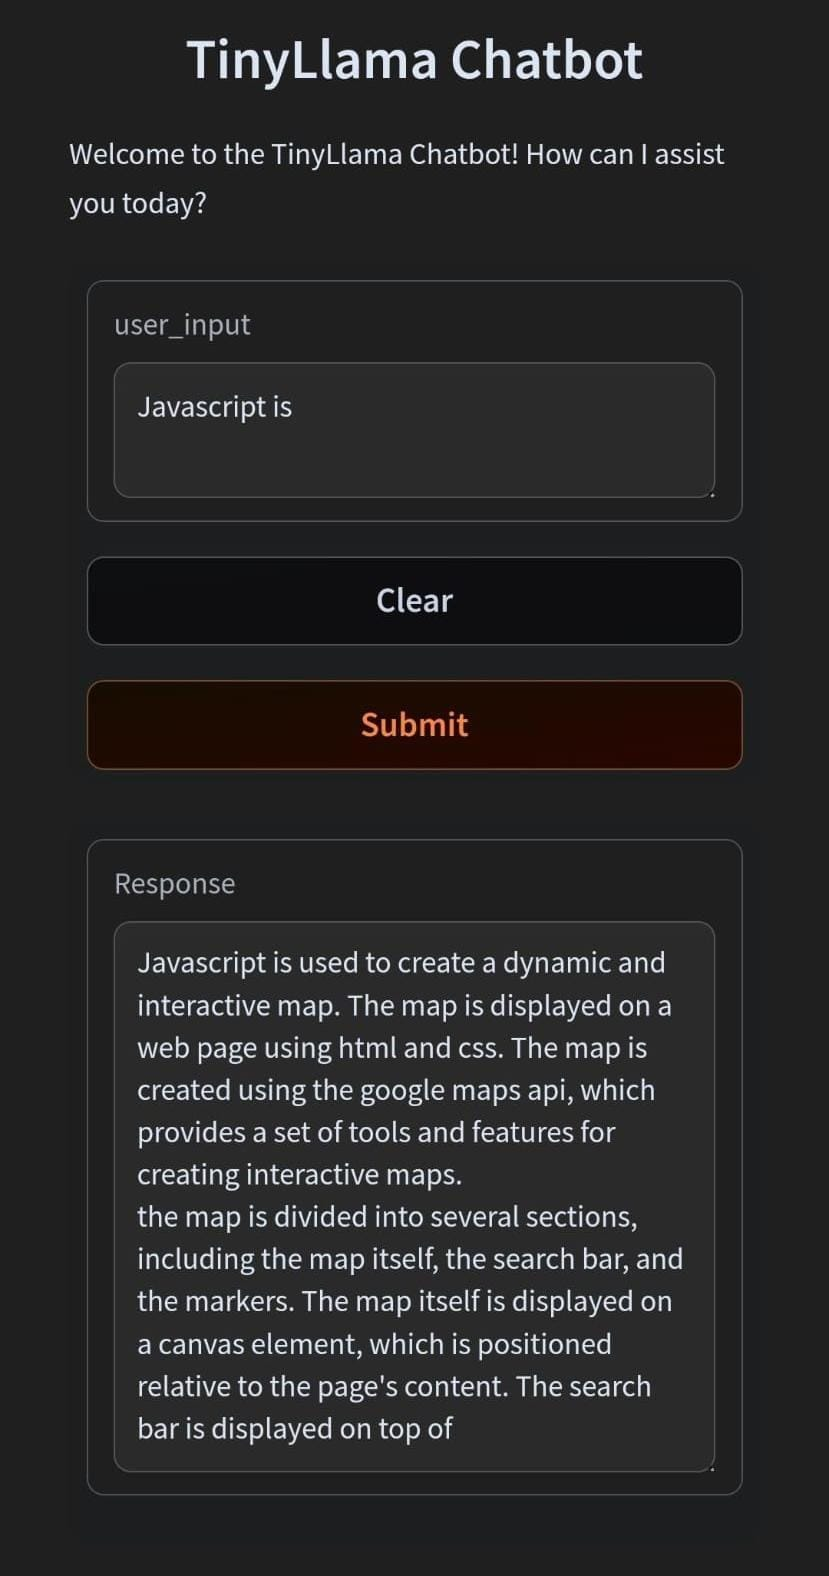
\includegraphics[width=\textwidth]{rep.jpg}
    \caption{Chatbot Response}
    \label{fig:inference}
\end{subfigure}
\caption{Gradio Interface}
\label{fig:model-comparison}
\end{figure}
\section{Results \& Discussion}
Converting the pre-trained TinyLlama model from PyTorch to ONNX ensures compatibility with tools like OpenVINO. Quantization reduces weights and activations to INT8, maintaining accuracy with calibration data. The model is exported to OpenVINO IR format, optimized for Intel hardware, validated for performance, and benchmarked to measure improvements in inference time, model size, and memory usage.


The comparison highlights the performance and resource utilization of an original machine learning model with its quantized version. The quantized model significantly improves inference speed, reducing the average time from 5.1595 seconds to 1.7184 seconds.The quantized model is also much more storage-efficient, reducing the model size from 4196.35 MB to just 1054.63 MB. This indicates that quantization effectively compresses the model, making it faster and more storage-efficient.
\begin{table}
\centering
\begin{tabular}{|c|c|c|c|c|}
\hline
Model No. & Model Name & Average Inference Time & Peak Memory Usage & Model size \\
\hline
1. & Tinyllama & 5.1595 s & 4018.65 MB & 4196.35 MB \\
\hline
2. & Optimized Tinyllama & 1.7184 s & 5046.84 MB & 1054.63 MB \\
\hline
3.& Meta Llama 3 & 0.8938 s & 141048.52 MB & 30633.02 MB \\
\hline
4.& Optimized Meta Llama 3 & 0.3338 s & 141053.06 MB & 7670.22 MB \\
\hline
\end{tabular}
\caption{Comparison of Model Performance}
\label{tab:model-comparison}
\end{table}

Table \ref{tab:model-comparison} shows a comparison between the original and optimized versions of the TinyLlama model, as well as the original and optimized Meta Llama models.

\begin{figure}[H]
\centering
\begin{subfigure}[b]{0.45\textwidth}
    \centering
    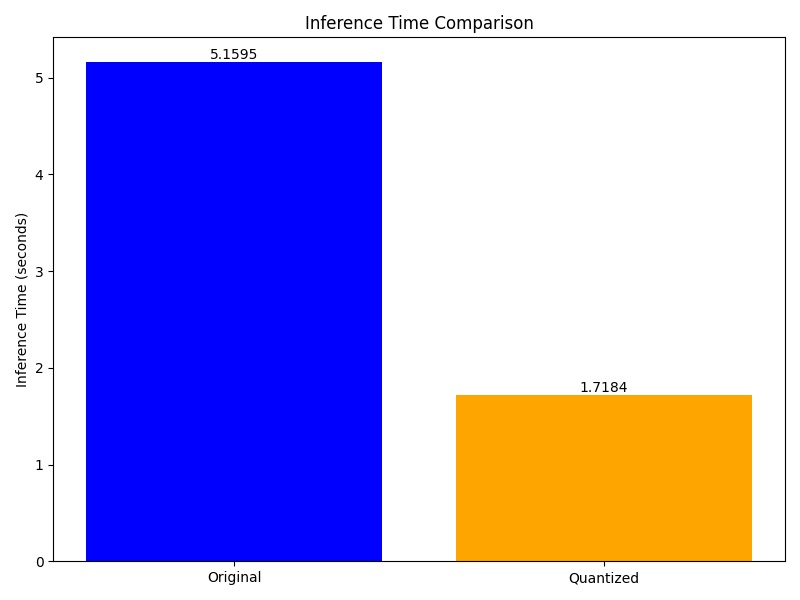
\includegraphics[width=\textwidth]{inf.jpg}
    \caption{Inference time comparison}
    \label{fig:inference}
\end{subfigure}
% Add your second subfigure here if needed
\begin{subfigure}[b]{0.45\textwidth}
    \centering
    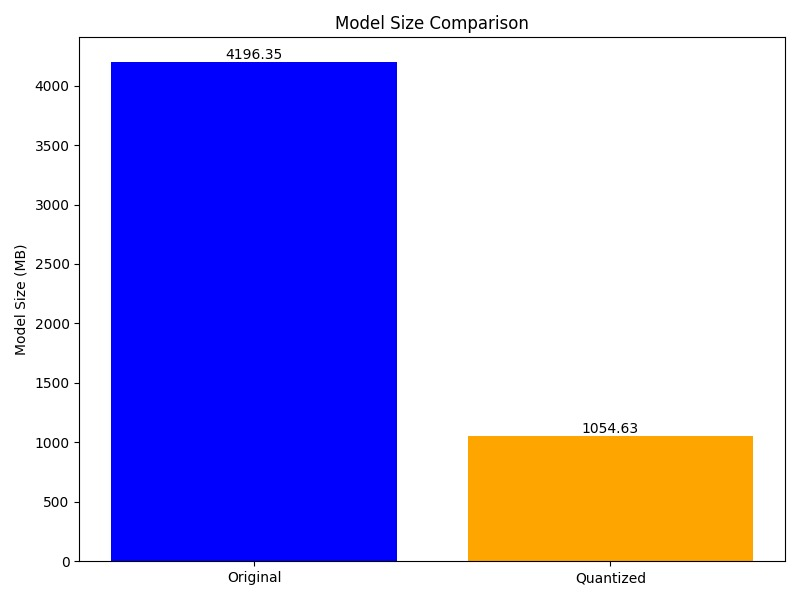
\includegraphics[width=\textwidth]{ms.jpg}
    \caption{Model size comparison}
    \label{fig:inference}
\end{subfigure}
\caption{Comparison of Models}
\label{fig:model-comparison}
\end{figure}

Figure 2. shows the comparison of original and optimized Tiny Llama model.
\section{Conclusion}
This project demonstrates the optimization and deployment of TinyLlama on Intel AI laptops using OpenVINO and NNCF. Through INT8 quantization and optimization, significant improvements in model size and inference speed were achieved while maintaining performance. An interactive chatbot showcases the practical application, highlighting the potential for running sophisticated AI models on consumer hardware. By balancing size, speed, and accuracy, this work contributes to AI democratization, making advanced language models accessible on Intel CPUs. The project addresses technical challenges and opens new possibilities for AI in resource-constrained environments, emphasizing the importance of hardware-software co-optimization in advancing AI accessibility.


Future research will focus on enhancing AI model performance on consumer devices through dynamic precision adjustment, multi-model integration, edge device optimization, improved fine-tuning, benchmarking, energy efficiency analysis,continuous learning capabilities, and cross-platform optimization. These efforts aim to improve AI adaptability, efficiency, and accessibility across diverse applications.
\section{Acknowledgments}
We would like to express our heartfelt gratitude and appreciation to Intel$^\copyright$ Corporation for providing an opportunity to this project.First and foremost, we would like to extend our sincere thanks to our team mentor Akshara Sasidharan for her invaluable guidance and constant support throughout the project.We are deeply indebted to our college Saintgits College of Engineering and Technology for providing us with the necessary resources,and sessions on machine learning. We extend our gratitude to all the researchers, scholars, and experts in the field of machine learning and natural language processing and artificial intelligence, whose seminal work has paved the way for our project. We acknowledge the mentors, institutional heads, and industrial mentors for their invaluable guidance and support in completing this industrial training under Intel$^\copyright$ -Unnati Programme whose expertise and encouragement have been instrumental in shaping our work.
\cite{*}
\bibliographystyle{josisacm}
\bibliography{josisexample}
\appendix
\section{Main code sections for the solution}
\subsection{Model Initialization and Conversion}
\begin{python}
model_name = 'TinyLlama/TinyLlama-1.1B-Chat-v1.0'
tokenizer = LlamaTokenizer.from_pretrained(model_name)
model = LlamaForCausalLM.from_pretrained(model_name)

# Export the model to ONNX format
torch.onnx.export(
    model,
    (dummy_input['input_ids'],),
    onnx_path,
    opset_version=14,
    input_names=["input_ids"],
    output_names=["output"]
)

# Convert the ONNX model to OpenVINO IR format
ov.serialize(onnx_model, ir_xml_path, ir_bin_path)
\end{python}
This section shows loading the original model, converting it to ONNX, and then to OpenVINO IR format.

\subsection{Model Quantization}
\begin{python}
nncf_config = {
    "input_info": {
        "sample_size": [1, 7]
    },
    "compression": {
        "algorithm": "quantization",
        "preset": "performance"
    },
    "quantizer": {
        "precision_bits": {
            "weights": 8,
            "activations": 8
        },
        "mode": "asymmetric"
    }
}

quantized_model = quantize(
    ov_model,
    calibration_dataset,
    preset=QuantizationPreset.PERFORMANCE
)

\end{python}
This part demonstrates the NNCF configuration for quantization and the actual quantization process.
\subsection{Performance Benchmarking}
\begin{python}
def get_file_size(file_path):
    return os.path.getsize(file_path) / (1024 ** 2)  # Size in MB

def benchmark_model(model, input_text, tokenizer, num_runs=10):
    inputs = tokenizer(input_text, return_tensors="pt")
    start_time = time.time()
    for _ in range(num_runs):
        outputs = model(**inputs)
    end_time = time.time()
    avg_time = (end_time - start_time) / num_runs
    return avg_time

def get_memory_usage():
    process = psutil.Process(os.getpid())
    return process.memory_info().rss / (1024 ** 2)  # Convert to MB

def benchmark_quantized_model(compiled_model, input_text, tokenizer, num_runs=10):
    inputs = tokenizer(input_text, return_tensors="pt")
    input_ids = inputs["input_ids"].detach().cpu().numpy()
\end{python}
These functions measure the inference time for both the original and quantized models.
\subsection{CPU Inference}
\begin{python}
core = Core() 
quantized_model = core.read_model(quantized_ir_path)
quantized_compiled_model = core.compile_model(quantized_model, "CPU")
# Print comparison results.
print(f"Original model - Average Inference Time: {original_model_time:.4f} seconds")
print(f"Quantized model - Average Inference Time: {quantized_model_time:.4f} seconds")
print(f"Original model - Peak Memory Usage: {original_model_memory:.2f} MB")
print(f"Quantized model - Peak Memory Usage: {quantized_model_memory:.2f} MB")
print(f"Original model size: {original_model_size:.2f} MB")
print(f"Quantized model size: {quantized_model_size:.2f} MB")


\end{python}
This section prints and visualizes the comparison results.
\subsection{Preprocessing and Postprocessing}
\begin{python}
def preprocess_text(text):
    text = text.lower()
    text = text.translate(str.maketrans('', '', string.punctuation))
    text = ' '.join(text.split())
    return text

def postprocess_response(response):
    response = response.strip()
    sentences = re.split(r'(?<!\w\.\w.)(?<![A-Z][a-z]\.)(?<=\.|\?)\s', response)
    sentences = [sentence.capitalize() for sentence in sentences]
    response = ' '.join(sentences)
    return response
\end{python}
These functions handle text preprocessing and response postprocessing.
\subsection{Chatbot Implementation}
\begin{python}
# Pipeline for text generation
pipe = pipeline("text-generation", model=model_path, tokenizer=tokenizer)
def generate_response(user_input):
    user_input = preprocess_text(user_input)
    response = pipe(user_input, max_length=100, temperature=0.7, top_k=50, top_p=0.9, num_return_sequences=1)[0]['generated_text']
    response = postprocess_response(response)
    return response

iface = gr.Interface(
    fn=generate_response,
    inputs=gr.Textbox(lines=2, placeholder="Input your message here..."),
    outputs=gr.Textbox(label="Response"),
    title="TinyLlama Chatbot",
    description="Welcome to the TinyLlama Chatbot! How can I assist you today?",
    examples=sample_prompts,
    theme="default",
    allow_flagging="never"
)
\end{python}
This shows how to use the optimized model for inference and create a Gradio interface for interaction.


\section* {Project Code:GitHub}
The project's code and other details related to the project are available in the following link:

\href{https://github.com/Rahul-Biju-03/Technix}{https://github.com/Rahul-Biju-03/Technix}

\end{document}


